\subsection{Nios II System}\label{subsec:CPU}
Der eingesetzte Nios II Prozessor ist für die Bedienung des Theremin und die Steuerung der Signalverarbeitungshardware zuständig. Die diversen eingesetzten IP Cores sind in den unten stehenden Kapiteln beschrieben.

\paragraph{JTAG, Timer und System ID}\mbox{}\\

Der JTAG IP Core ermöglicht das flüchtige Programmieren des Nios II wie auch das Kommunizieren mit selbem für Debugging Zwecke. 
Durch den Einsatz des Timer IP Cores erhält der Nios II einen Interval Timer, um beispielsweise periodisch Interrupts zu generieren. 
Im System ID IP Core ist die Systemidentifikationsnummer gespeichert. Diese ist nötig, um beim Laden der Software sicherzustellen, dass das passende Hardware Image vorhanden ist.
Alle drei Komponenten sind mit Standardeinstellungen in das Nios II System eingefügt worden.

\paragraph{Speicher}\mbox{}\\

Der Arbeitsspeicher ist ein externer 64MB SDRAM Chip IS42S16320D von ISSI. Für die Kommunikation mit dem Nios II Prozessor ist der SDRAM Controller IP Core zuständig. Der Nios II Prozessor kann über das Memory Mapped Interface mit dem Core kommunizieren und so auf das SDRAM zugreifen. Da dieser Chip bereits auf dem Entwicklungsboard vorhanden ist und um Ressourcen zu sparen, haben wir uns gegen On-Chip Speicher entschieden.\\

Das Hardware Image und der Programmcode sind auf dem Board enthaltenen Flash Speicher gespeichert. Dabei lädt Quartus, anders als bei dem nicht flüchtigen Programmieren, nicht das SRAM Object File (.sof) sondern ein JTAG Indirect Configuration File (.jic). Das Erstellen dieses Files geschieht im Quartus aus dem SRAM Object File und dem in Eclipse generierten HEX File. Der USB Blaster lädt das .jic File über ein Serial Flash Loader Image auf den Flash Speicher. Das FPGA kopiert beim Einschalten des Gerätes zuerst das Hardwareimage und anschliessend den Programmcode. Auf Empfehlung von Dokumentationen von Intel haben wir uns entschlossen, den Programmcode durch einen Bootcopier ins SDRAM zu kopieren. Abbildung \ref{img:FlashLayout} zeigt das Layout des Flash Speichers nach dem Programmieren \cite{non_volatile}.

\begin{figure}[h!]
	\centering
	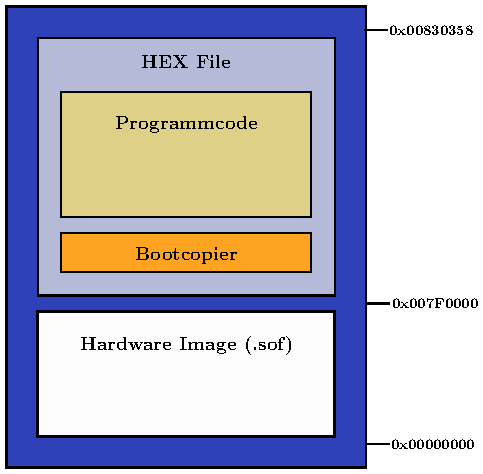
\includegraphics[width=0.45\textwidth]{FlashLayout.pdf}
	\caption{Layout des Flash Speichers} 
	\label{img:FlashLayout}
\end{figure}  

\paragraph{LCD Controller \& Reset}\mbox{}\\

Für das beschreiben des LCD ist die von Terasic bereitgestellte VHDL Komponente\\ LT24\_Controller zuständig. Der Nios II Prozessor steuert diese über das Memory Mapped Interface. Das verwendete Display LT24 von Terasic enthält für das Schreiben des LCD den LCD Treiber ILI9341 von ILITEK. Dieser Chip wird durch den LT24\_Controller über das parallele \SI{16}{Bit} Interface gesteuert. Weiter kann der LCD Chip über den PIO Core LCD Reset zurückgesetzt werden. Wie diese beiden Komponenten in Software angesteuert werden ist in Kapitel \ref{subsec:drivers} genauer beschrieben \cite{LCD_Chip}.

\newpage

\paragraph{Touchscreen}\mbox{}\\

Der Touch Screen Digitizer AD7843 von Analog Devices misst den resistiven Touchscreen des LCD aus und übermittelt die digitalisierten Koordinaten über SPI an den Prozessor. Der Nios II kommuniziert dabei über drei verschiedene IP Cores mit diesem Chip: Der SPI Core \textit{Touch SPI} für die Datenübertragung, der PIO Core \textit{Touch Busy} um den Beschäftigungsstatus des Chips abzufragen und den zweiten PIO Core \textit{Touch Interrupt}, welcher den Nios II über eine Betätigung des Touchscreens informiert. Bei einer Berührung des Touchscreens löst \textit{Touch Interrupt} beim Nios II Prozessor einen Interrupt aus, welcher sofort die Koordinaten über SPI anfordert \cite{Touch_ADC}.